\documentclass[aip,apm,amsmath,amssymb,reprint]{revtex4-2}

\usepackage[utf8]{inputenc}
\usepackage[T1]{fontenc}
\usepackage{mathptmx}
\usepackage[scaled=0.9]{couriers}
\usepackage{xcolor}
\usepackage{graphicx}
\usepackage{hyperref}

\frenchspacing

\begin{document}

\title{Machine learning approaches for the prediction of materials properties}

\author{S. Chibani}
\author{F.-X. Coudert}
\email{fx.coudert@chimieparistech.psl.eu}
\affiliation{Chimie ParisTech, PSL University, CNRS, Institut de Recherche de Chimie, Paris, 75005 Paris, France}

\date{\today}

\begin{abstract}
We give here a brief overview of the use of machine learning in our field, for chemists and materials scientists with no experience with these techniques. We illustrate the workflow of machine learning for computational studies of materials, with specific interest in the prediction of materials properties. We present concisely the fundamental ideas of machine learning, and for each stage of the workflow give examples of the  possibilities and questions to consider in implementing ML-based modelling.
\end{abstract}

\maketitle

\section{Introduction}

The pace of systematic materials discovery has quickened in the last decade. The number of studies systematically exploring various families of materials, with the goal of discovering existing materials with unsuspected properties, or designing novel materials with targeted properties, is growing at an astounding rate. Databases of experimental structures --- in particular crystalline structures --- continue to grow at a steady pace, and are complemented with larger and larger databases of physical and chemical properties. High-throughput experiments and combinatorial materials synthesis are aided by robotics and artificial intelligence, performing reactions and analysis faster. On the computational side of things, molecular simulations have expanded in scale, allowing scientists to predict structure and properties of complex materials even before they are synthesized. The prediction of compounds properties with high accuracy can be coupled with high-throughput screening techniques, to help search for new materials. Yet, despite the advances in the computational power, computational methods --- whether at the quantum or classical level --- are still relatively time consuming and can hardly explore the properties of all possible chemical compositions and crystal structures. In order to reach this goal of systematic exploration of chemical space, and to help leverage the large-scale databases of structures and properties that are nowadays available, computational chemistry and materials science are turning more and more often to machine learning (ML), a subset of artificial intelligence (AI) that has seen tremendous developments in the recent years and widespread application across all fields of research.

The main idea of artificial intelligence emerged in the 1950s when Alan Turing wondered if a machine could ``think''.\cite{TURING1950} The term of ``artificial intelligence'' (AI) was first coined by John McCarthy in 1955, and is defined as the set of theories and techniques implemented in order to create machines capable of simulating intelligence. In other words, AI is the endeavour to replicate the human intelligence in computers. In 1959, Arthur Samuel produced computer programs that were playing checkers (draughts) better than the average human, and that could learn to improve from past games.\cite{Samuel1959} Since then, AI and data-intensive algorithms have seen such an important development that they are sometimes called the ``fourth paradigm of science''\cite{Hey2009} or the ``fourth industrial revolution''. AI is now routinely used in different fields: face recognition, images classification, information engineering, linguistics, psychology, medicine, and it has impact in the fields of philosophy and ethics.

AI-powered machines are usually classified under two broad categories: general and narrow. The artificial general intelligence (AGI) is a machine that can learn to solve any problem that the human intellect can solve. Also referred to as ``strong AI'' or ``full AI'', it is currently hypothetical, the kind of artificial intelligence that we see in the science fiction movies. The creation of AGI is an important goal for some AI researchers, but is an extremely difficult quest and generally considered too complex to be achieved in the near future.\cite{2007} In contrast, narrow AI (or ``weak AI'') is a kind of artificial intelligence focussed on performing specific tasks, defined in advance. Narrow AI has seen a very large number of successful realizations of artificial intelligence to date, sometimes in applications where the machine seems intelligent (in the human way), and sometimes hidden under the hood. Much of these successes of narrow AI have been made possible by advances in machine learning (ML) in general, and in deep learning (DL) more specifically in the past few years.

Machine learning aims at developing algorithms that can learn and create statistical models for data analysis and prediction. The ML algorithms should be able to learn by themselves --- based on data provided --- and make accurate predictions, without having been specifically programmed for a given task. Beyond theoretical developments, recent years have seen rapid advances in the application of machine learning, not only by computer scientists and experts in the development of AI algorithms, but also by other researchers in different fields who adopt these techniques for their own purposes. Among many other fields of research, chemical and materials sciences have been impacted by the application of machine learning to accelerate certain computational tasks, or to solve problems for which traditional modelling methods were ill-suited. Deep learning, a subset of machine learning based on artificial neural networks, promises to escalate the advances of AI even further.

\begin{figure*}[t]
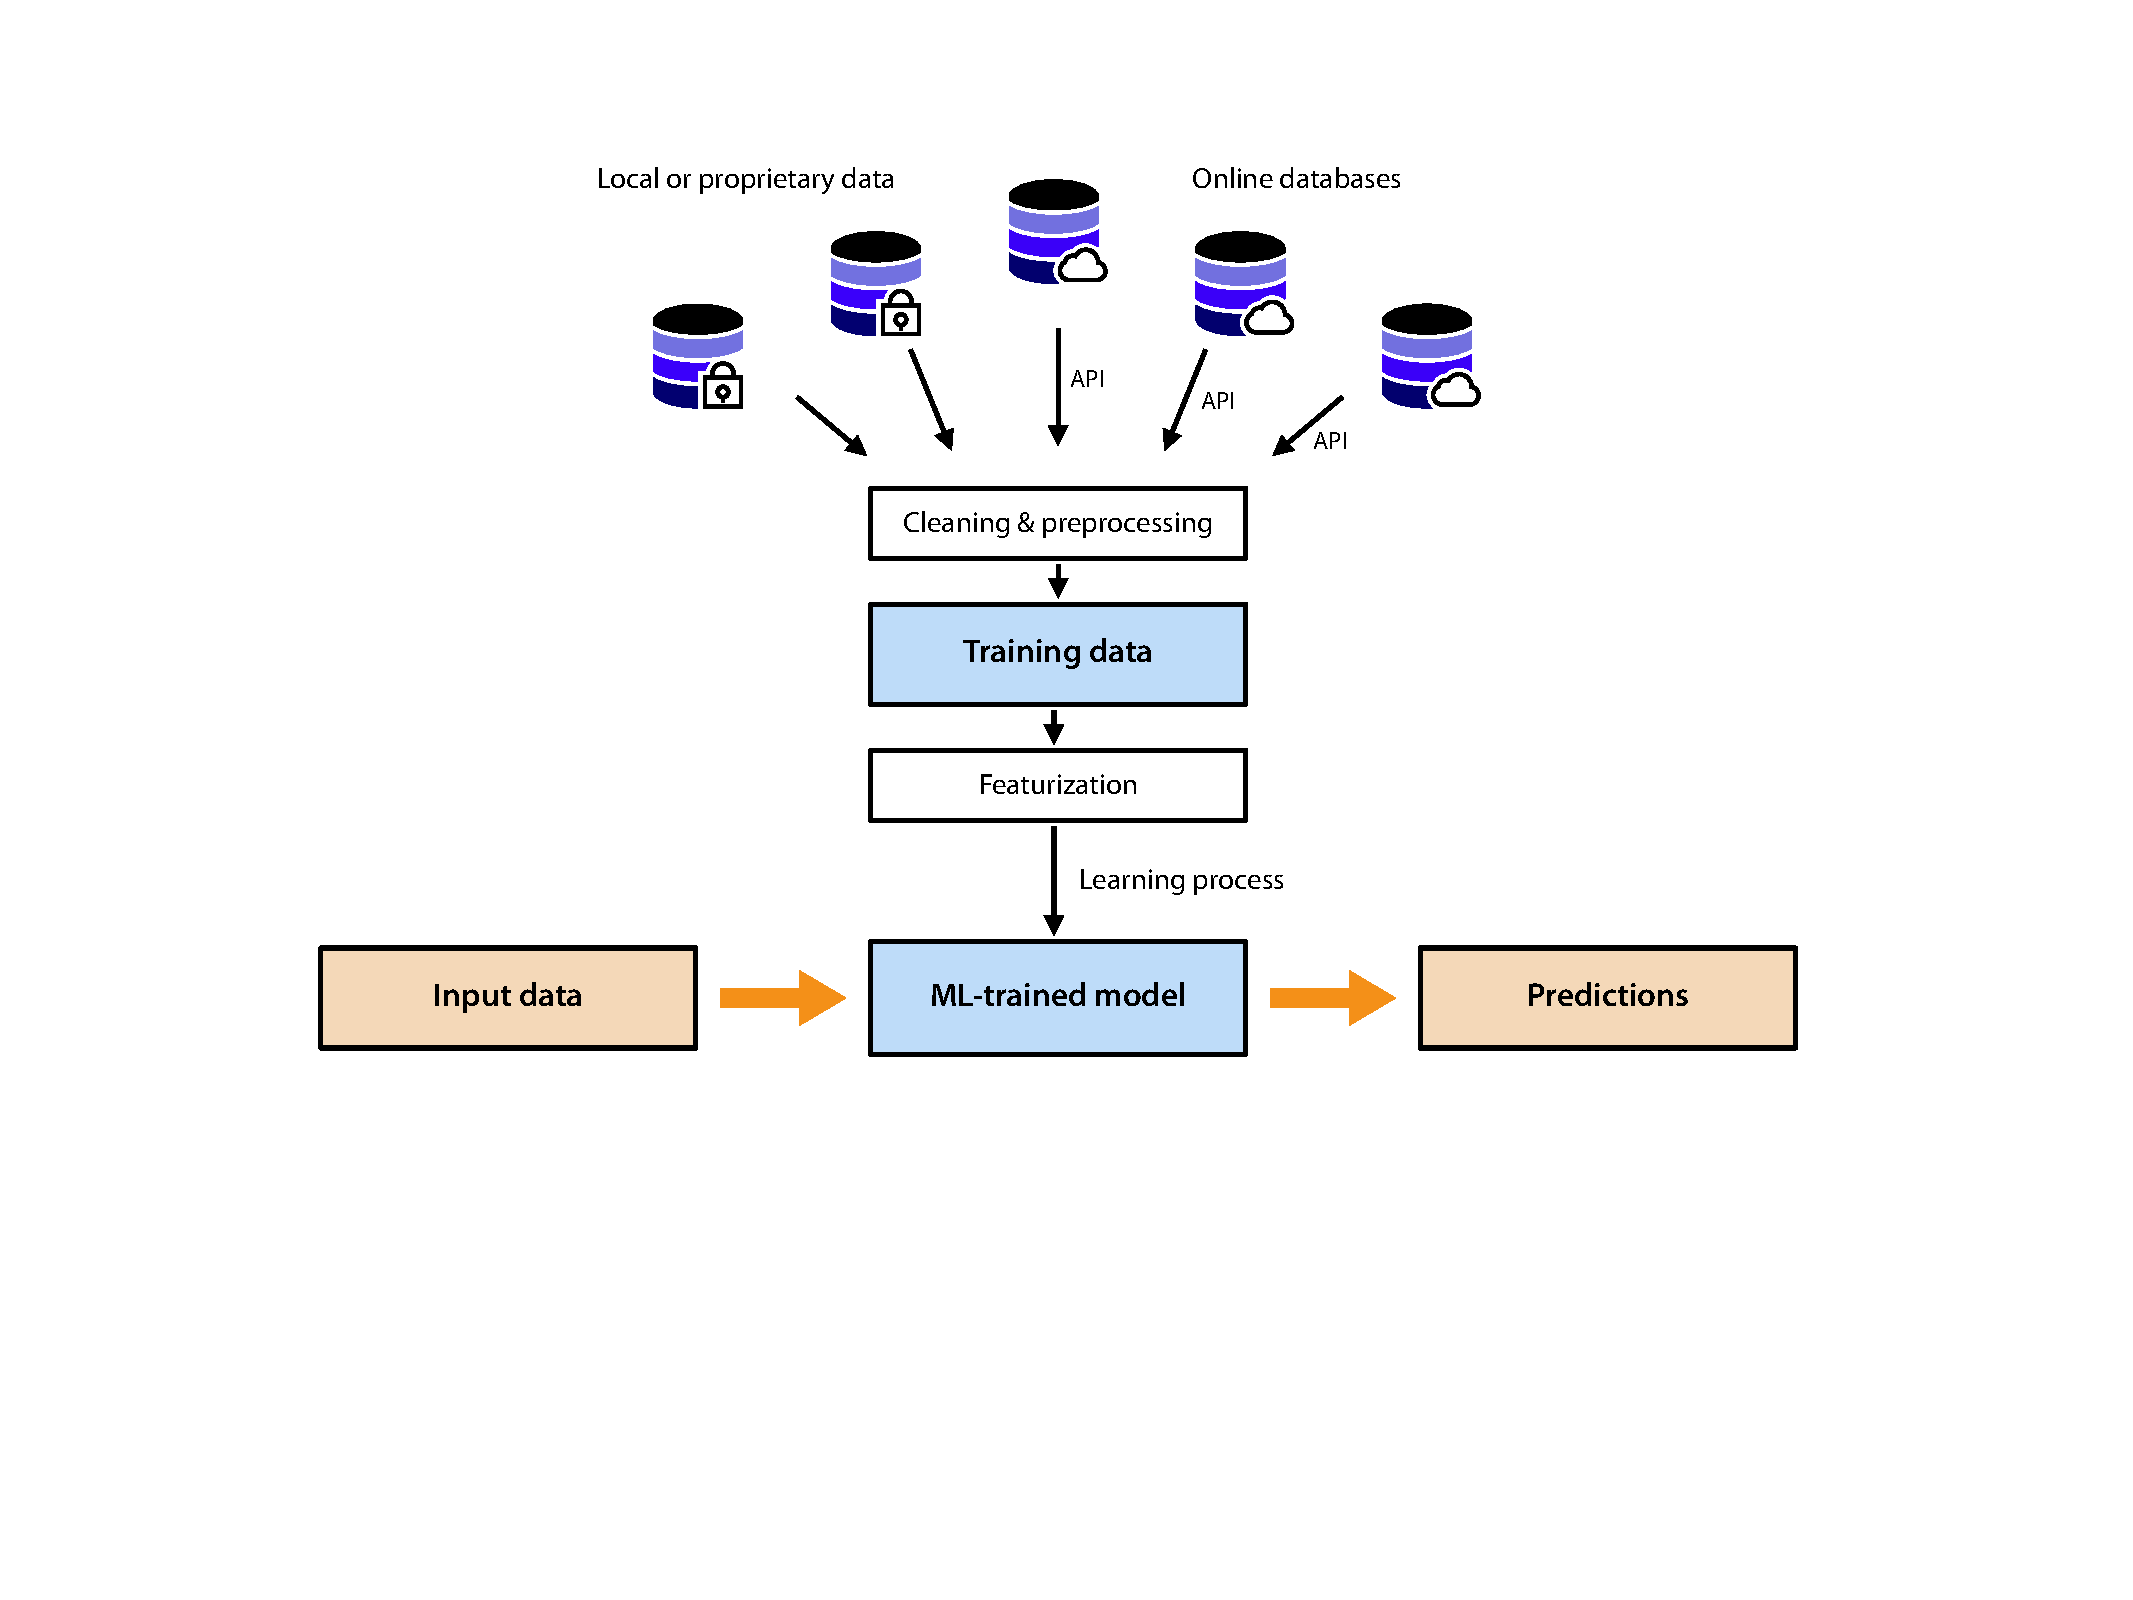
\includegraphics[width=13cm]{ML_workflow}
\caption{\label{fig:ML_workflow} Simplified overview of a machine learning workflow. The machine learning model is trained on input data gathered from multiple databases. Once it is trained, it can be applied to make predictions for other input data.}
\end{figure*}

In this paper, we set out to illustrate the workflow of machine learning in a computational materials context, and give examples at each stage of the possibilities and questions to consider in implementing ML-based modelling. In this very active and rapidly expanding field of research, we will try to highlight some --- but not all --- of the machine learning techniques have been successfully applied in real applications for computational chemistry of materials, either as they are representative of what is done in the field, or because they represent recent and exciting developments. We will also discuss the specific contributions made to our field by deep learning studies, although they are currently more limited. The goal of this paper is to provide a brief overview to chemists and materials scientists, but we do not try to be exhaustive in our discussion of the state of the art. For a full review on machine learning for molecular and materials science, we refer the reader to the excellent introductory yet thorough review of Butler et al.\cite{Butler2018}


\section{Implementing a machine learning methodology}

\begin{table*}
    \centering
    \setlength\tabcolsep{10pt}
    \begin{tabular}{lll}
\textbf{Database} & \textbf{Structures} & \textbf{Properties} \\[2mm]
\emph{Structural databases} \\\hline
Cambridge Structural Database (CSD)              & 1,031,632 \\
Inorganic Crystal Structure Database (ICSD)      & 218,839 \\
Crystallography Open Database (COD)              & 457,771 \\
International Centre for Diffraction Data (ICDD) & 1,004,568 \\[2mm]
\emph{Databases of structures and properties} \\\hline
AFLOW             & 3,249,264    & Formation energy, band structures, Bader charges \\
                  &              & Elastic \& thermal properties \\
                  &              & Binary, ternary, quaternary systems \\
Materials Project & 654,758      & Band structures \\
                  &              & Elastic \& piezoelectric tensors \\
                  &              & Porous volume and surface \\
Open Quantum Materials Database (OQMD)
                  & 637,644      & Formation energy, band structures \\

    \end{tabular}
    \caption{Some of the largest and most-used databases in materials sciences, broken down in two categories: databases restricted to crystalline structures only, and databases focused on both structures and materials properties.}
    \label{tab:repositories}
\end{table*}


\subsection{Gathering data}

As stated in the introduction, machine learning algorithms are trained on existing datasets to learn and improve. In order to create accurate models, the size and quality of the datasets used for training plays a crucial role. This identification, gathering or creating (in some cases) of the training dataset is the first step of machine learning workflow, and will of course heavily depend on the goal of the model you want to train. For generic purposes, in order to ``learn by doing'' the various steps in implementing a ML workflow, one can find free datasets through platforms like Kaggle (\url{https://www.kaggle.com}), the UC Irvine Machine Learning Repository (\url{https://archive.ics.uci.edu/ml}), or on governmental or agency websites that gather and promote open data (\url{https://www.data.gouv.fr} in France, \url{https://www.data.gov/} in the United States).

When it comes to materials sciences, there are a number of available datasets that have been published and validated in the scientific literature. Many of them are open and publicly available to any potential user, but others have stricter licensing terms or require a paid subscription for access to some or all features. On practical terms, they mainly differ in the data featured within the dataset, with two main categories: databases that focus (exclusively or predominantly) on structural information, and databases that focus on physical or chemical properties of materials. Table~\ref{tab:repositories} presents a short list of selected databases in materials sciences.

The first category, \emph{i.e.} databases of structures of materials, is probably the most well-known and historically the most developed. They include the ubiquitous Cambridge Structural Database (CSD, \url{https://www.ccdc.cam.ac.uk}), featuring more that one million experimental crystal structures, and which is considered a standard repository for the publication of new crystal structures ranging from organic, metal--organic and organometallic molecules and compounds. Other such databases include the Inorganic Crystal Structure Database (ICSD, \url{https://icsd.fiz-karlsruhe.de}) for inorganic crystals, the freely accessible Crystallography Open Database\cite{Grazulis2009} (COD, \url{http://crystallography.net}), the International Centre for Diffraction Data (ICDD, \url{http://www.icdd.com/}), and many others. Similar databases exist for other chemical systems, such as GDB\cite{Fink2007} (\url{http://gdb.unibe.ch/downloads/}) for small organic molecules, and ZINC\cite{Sterling2015} (\url{https://zinc15.docking.org/}) for commercially-available compounds for virtual screening.

As it appears readily while reading the above list, it is important to be aware of an important bias in how these databases cover the field of materials science: they are all limited to crystallographic structures. While this is obviously linked to the nature of the determination of the structure and its representation, it is important to be aware of such a bias. It is only one example --- and there are many others --- of how databases exhibit, by the very own choice of their scope and the representations chosen, a biased representation of the wide scope of the field of materials sciences. It is therefore necessary to be aware of the biases in the datasets one is using, both implicit and explicit.

Beyond structural databases, the past few years have seen the development of another category, with a rapid growth in the number of structure–property databases available --- often, again, with a specific focus on a particular class of materials or specific properties. The existence of such databases with a large amount of data, most of which are open access and collaborative, presents significant opportunity to train and to validate new machine learning models. We list some here, whose characteristics are summarized in Table~\ref{tab:repositories}; the choice made is not to try and be exhaustive (which would necessarily fail, given the large and ever-growing number of existing databases), but to highlight those that appear commonly used and have easy access and are well-documented for newcomers to the materials discovery field. Among the largest databases, we can cite the Materials Project\cite{MaterialsProject} (\url{https://materialsproject.org/}) for inorganic materials, the AFLOWLIB\cite{AFLOW} ``Automatic Flow for Materials Discovery'' (\url{http://aflowlib.org/}), and the Open Quantum Materials Database\cite{OQMD} (\url{http://oqmd.org}). In addition to these generic sources, there are also specific databases of computed properties for specific classes of materials, such as the Harvard Clean Energy Project\cite{Hachmann2011} (previously at \url{https://cepdb.molecularspace.org}, currently being migrated) for organic solar materials, TE Design Lab\cite{Gorai2016} (\url{http://tedesignlab.org}) for thermoelectric materials, NREL Materials Database\cite{Stevanovic2012} (\url{https://materials.nrel.gov}) for renewable energy materials. Finally, other online portals allow the sharing and exchange of computational data on materials from different origins, resulting in a more heterogeneous dataset, such as the Materials Cloud\cite{MaterialsCloud} (\url{https://www.materialscloud.org/}).

Most of these databases are accessible through both a web front-end, for simple exploration and visualization purposes, and an Application Programming Interface (API). An API is a web interface with well-documented behavior, whose queries and results are machine-readable in a agreed-upon format, making them well-suited for automated exploitation. These API are typically accompanied with a software layer to facilitate integration into projects, such as the Python Materials Genomics (\texttt{pymatgen})\cite{Ong2013} Python package that integrates with the Materials Project RESTful API, or the Automated Interactive Infrastructure and Database (AiiDA).\cite{Pizzi2016}

Finally, we would be remiss if we did not note that it is also possible to generate data to form a machine learning training set ``on the fly'', by performing high-throughput calculations on materials of interest. When this is done, it is then expected that the dataset produced is published alongside the work, as supporting information or submitted to an online data repository.


\subsection{Cleaning and preprocessing data}

We have described above how to use existing datasets of materials structures and properties (or generate one's own), yet this data cannot be used directly in the original format, and loaded ``as is'' in a machine learning workflow. When it comes to large datasets, four points are considered crucial in big data workflows, called the ``four V's'', and they are also relevant in machine learning methodologies: (i) \emph{volume}, the amount of data available, ; (ii) \emph{variety}, the heterogeneity of the data in both form and meaning; (iii) \emph{veracity}, the knowledge of the uncertainties associated with each data point; and (iv) \emph{velocity}, how fast the data is generated and has to be treated --- not usually an issue in our workflows, which do not have to work in real time.

Therefore, data has to be homogeneized and cleaned before it can be used. This means identifying possible erroneous, missing, or inconsistent data points (outliers), using criteria based on physical or chemical knowledge. This cleaning and homogeneization of the data is a key step in order to build more accurate predictors through machine learning. The need for this may depend on the workflow followed: for example, some ML algorithms are more robust than others in the presence of outliers. Some algorithms (like the Random Forest family) do not support null values in their input, while others can handle those.

To give one example of the necessity of this curation of the training data set, we recently performed a large-scale exploration of the elastic properties of inorganic crystalline materials available on the Materials Project database. By analyzing the elastic data present, we quantified that, out of 13,621 crystals, only 11,764 structures were mechanically stable, while 1,857 (around {14\%} of materials in the database) had elastic tensors that indicated mechanical instability (and were therefore unusable for further analysis).\cite{Chibani2019} Other materials had elastic moduli that were mathematically acceptable but unphysically large, and those needed to be removed as well before using the dataset.

\subsection{Representing data}

Once data has been cleaned up and homogeneized, the next step in the machine learning workflow is the encoding of this data into a set of specific variables, that will be manipulated directly by the ML algorithm. The data collected are often in a raw format and will need to be converted into a format suitable to learning procedure, usually as a series of scalar or vector variables for each entry of the dataset. This step can include the transformation of existing data (such as physical properties) by rescaling, normalization or binarization to bring it to such a state that the algorithm can easily parse it. Some basic pre-processing techniques are widely available in ML software, such as the \texttt{MinMaxScaler} or \texttt{StandardScaler} methods in scikit-learn.\cite{scikit-learn} In all cases, the effect of this preprocessing of the data needs to be studied carefully: it is important to mention that sometimes algorithms can deliver better results without preprocessing, and with excessive preprocessing it may not be possible to identify the crucial features that will give the best performance for the target variable.

When the input data consists of chemical structures, the choice of representation of the data is not always obvious: chemical compounds and materials are complex three-dimensional objects, whose direct representation as vectors of coordinates may not be efficient as input for the ML workflow. This question of the best representation of the data for the learning algorithm is called \emph{featurization}, or feature engineering. It is a very active area of research, in particular when it comes to describing chemical structures. The two main goals of feature engineering are: (i) preparing the input data in a form that the ML algorithms will work well with (and that can depend on the specific characteristics of the algorithm chosen); (ii) improving the performance of ML models, by using our knowledge of the materials and their important features (chemical intuition) in the building of the input data.

The chemical information about a given system can then be transformed into a series of so-called descriptors, that encode the chemical information, creating a new input that should describe the key features of the dataset in a way that allows for the ML algorithm to train efficiently. Many different mathematical representations are used as descriptors for chemical and materials structures (and their properties). We will cite here examples for molecular structures such as Coulomb matrix,\cite{Rupp2012} SMILES,\cite{Weininger1988} bag of bonds,\cite{Hansen2015} molecular graphs\cite{Faber2017} and BAML (using bonds, angles, and higher order terms)\cite{Huang2016}. Among the representations used for crystals, we find representations such as translation vectors, fractional coordinates of the atoms, radial distribution functions,\cite{Schtt2014} Voronoi tessellations of the atomic positions,\cite{Ward2017} and property-labelled materials fragments.\cite{Isayev2017}

\subsection{Machine learning models}

\subsubsection{Supervised learning}

Let us now move to fourth step of the machine learning workflow: the ``learning'' part itself, \emph{i.e.}, the training of the ML algorithm. Using the curated and pre-processed dataset as input, there are then three main categories of ML models: supervised, unsupervised, and semi-supervised. In \emph{supervised learning}, the dataset is considered as a training set, and must contain both input variables and their corresponding output variable: think of chemical structures and their properties, for a common example in chemistry. Then the goal of the ML algorithm is to learn, from this training data, the mapping function from the input (the structures) to the output (the properties). The main goal of the machine learned algorithm in a supervised learning approach is to be able to make a prediction for new data, with an acceptable level of accuracy, once it has been trained.

It is useful to know that supervised learning problems can be broadly categorized into two main types: regression and classification techniques. Both of them have as goal the construction of a model that can predict values from the available variables. The only difference between the two is type of output variable: in a regression-type prediction problem, the variable that is to be predicted is continuous, taking real values: melting point, band gap, elastic modulus, etc. Regression learning algorithms include linear regression, lasso linear regression, ridge regression, elastic net regression, Gaussian progresses regression, and classification and regression trees. The simplest of these algorithms is the linear regression (LR), which --- similarly to the common linear regression in 2D graphs --- tries to create the best linear model based on the descriptors given. If the model is complex, a lasso linear regression algorithm can be used instead, which is a modification of LR where the loss function is modified to minimize the complexity of the model.

On the other hand, for classification problems, the algorithm has to predict a categorical variable, \emph{i.e.} attribute a label to the input data. In the simplest case, these categories are reduced to two in a binary variable, such as: is the material conducting or isolating? is it porous or not? (or in another context: is this email a spam or not?) A large number of different classification algorithms can be used: logistic regression, linear discriminant analysis, $k$-nearest neighbour, naive Bayes, classification and regression tress, support vector Machine and kernel ridge regression (KRR). To given an example, Ghiringhelli et al. used KRR with descriptors derived from the energy levels and radii of valence orbitals to predict crystalline arrangements between zinc blende and wurtzite-type crystal structures.\cite{Ghiringhelli2015}

\begin{figure}[t]
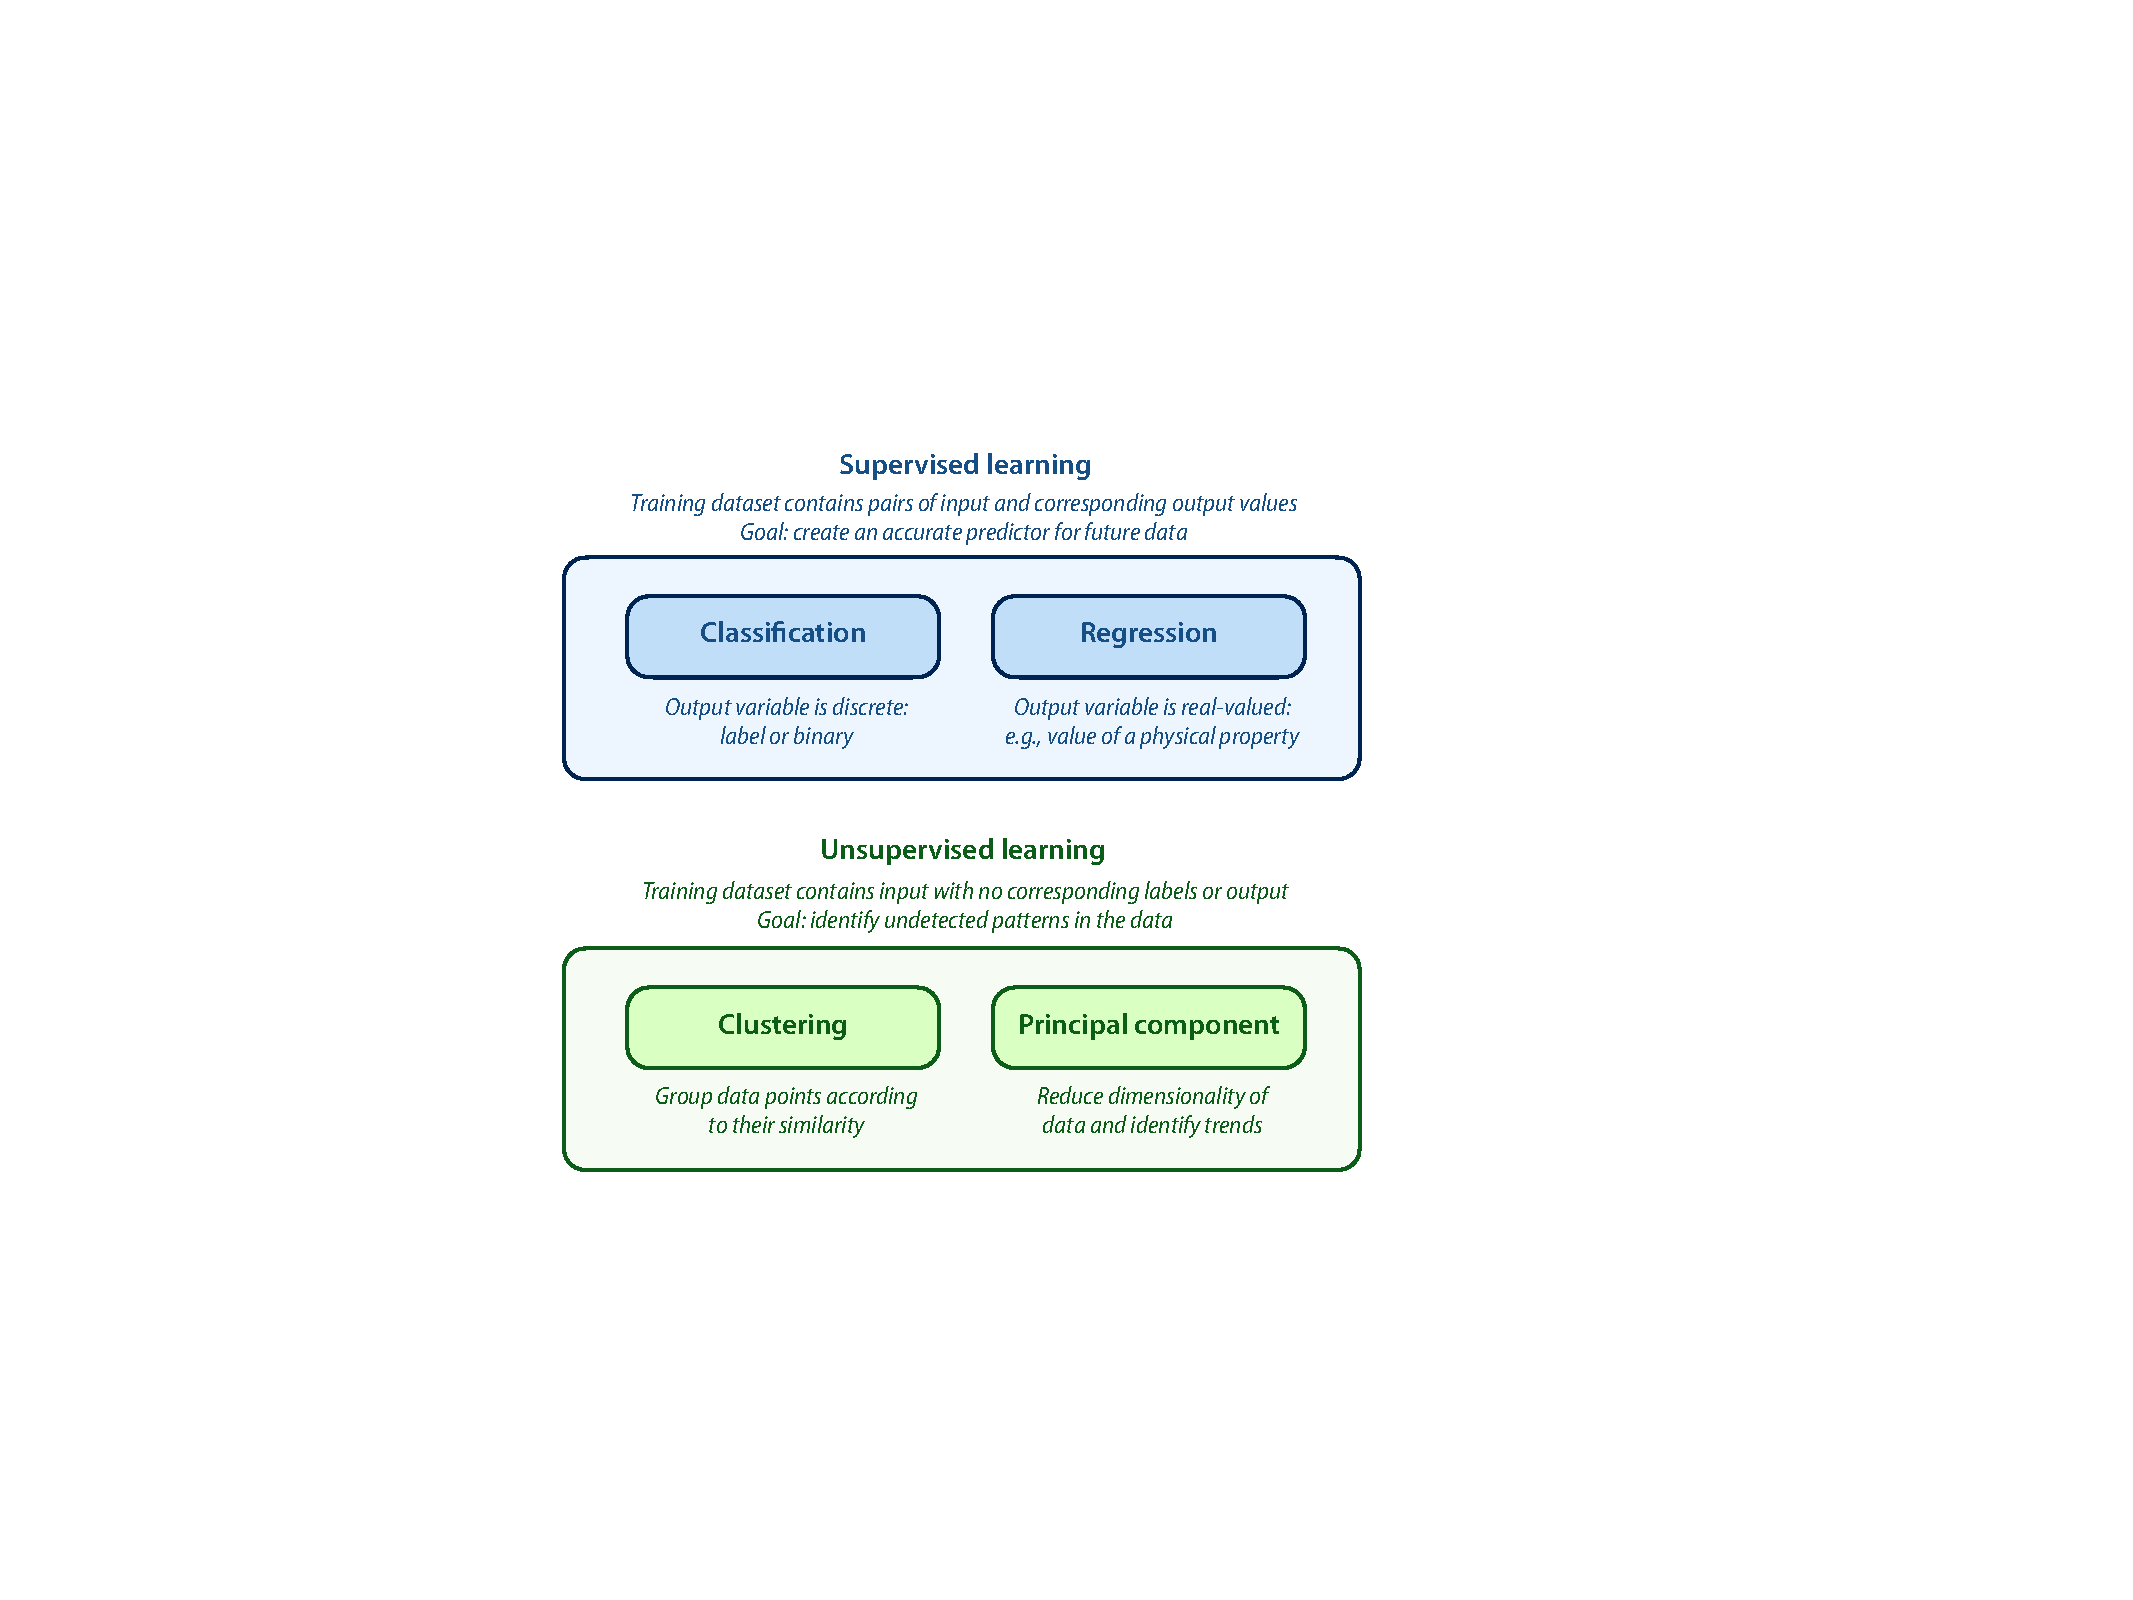
\includegraphics[width=85mm]{categories}
\caption{\label{fig:ML_categories} Different categories of machine learning models.}
\end{figure}


\subsubsection{Unsupervised learning}

\emph{Unsupervised learning} works in a completely different way, trying to draw inferences about the input data without any corresponding output variables: it is used to look for previously undetected patterns in data with minimal human supervision or guidance. It can, for example, act on unlabelled data to discover the inherent groupings. The ML algorithm tries to identify trends that could be of interest to rationalize the dataset, and present the available data in a novel way. One family of unsupervised learning algorithm is the clustering, or cluster analysis: there the ML workflow will split the data in several groups (or clusters) of records presenting similar features, without no prior assumption on the nature of these groups (unlike, for example, in supervised learning classification tasks). Classical methods used for clustering include Gaussian mixtures, $k$-means clustering, hierarchical clustering, and spectral clustering. Another type of unsupervised learning method are association rule learning and principal component algorithms, that aim to establish relationships between multiple features in large dataset, something that is difficult to do by hand. Popular algorithms for generating association rules have been proposed, such as Apriori, Eclat and FP-Growth.

When it comes to applications in chemistry and materials science, supervised machine learning is a lot more common, but there are some examples of unsupervised learning nonetheless; for a recent perspective on this specific topic, see Ref.~\citenum{Ceriotti2019}. Saad et al. applied both supervised and unsupervised ML techniques to predict the structure and properties of crystals (such as melting point) for binary compounds.\cite{Saad2012} Supervised ML models have been trained to reproduce the LUMO and HOMO for organic solar cells,\cite{Pereira2016} and to predict key thermodynamic parameters such as adsorption energy,\cite{Toyao2018} activation energy,\cite{Takahashi2018} and active site\cite{Jinnouchi2017} in catalytic processes. Isayev et al. developed predictive Quantitative Materials Structure-Property Relationships (QMSPR) models through machine learning, in order to predict the critical temperatures of known superconductors,\cite{Isayev2015} and Woo and coworkers established QMSPR model to achieve high-throughput screening of metal--organic frameworks (MOFs) to capture CO\textsubscript{2} by adsorption, relying on machine learning to explore the large dimensionality spanned by their exceptional structural tuneability.

One disadvantage of supervised ML algorithms lie in the acquisition of labeled data, an expensive process requiring especially when dealing with large amounts of data. Unlabeled data, on the other hand, is relatively inexpensive and easy to collect and to store --- but applications are unsupervised ML in materials sciences have been relatively limited. An alternative exists, in the form of a third training ML model named \emph{semi-supervised}, which is halfway between supervised and unsupervised learning, as its name implies. In such a workflow, we have a large amount of input data and only a limited amount of corresponding output data. Semi-supervised ML aims at learning from the labeled part of the dataset, training an accurate model. First, the workflow will uses unsupervised learning algorithm to identify and cluster similar data. Then, it will use supervised learning techniques to train and make prediction for the rest of the unlabeled data. Semi-supervised learning algorithms make three assumptions about the data, which somewhat restrict their applicability: (i) continuity assumption: the close points are more likely to share a label; (ii) cluster assumption: data can form discrete clusters and points in the same cluster are more likely to share an output label; (iii) manifold assumption: the data lie approximately on a manifold of much lower dimension than the input space. Semi-supervised algorithms are widely used in text and speech analysis, internet content classification and protein sequence classification applications.

Semi-supervised learning was used by Court et al. to create a materials database of Curie and N{\'e}el temperatures for 39,822 by text mining a corpus of 68,078 chemistry and physics articles, applying natural language processing and a semi-supervised relationship extraction algorithm to obtain the values (and units) of the properties from the texts.\cite{Court2018} Similarly, Huo et al. demonstrated the efficiency and accuracy of semi-supervised machine-learning to classify inorganic materials synthesis procedures from written natural language.\cite{Huo2019} Recently, Kunselman et al. used semi-supervised learning methods to analyse and classify microstructure images, training their model on a dataset where only a fraction of the microstructures was labeled initially.\cite{Kunselman2020}


\subsubsection{Applications}

Most of the applications of ML in chemical and materials sciences, as we have said, feature supervised learning algorithms. The goal there is to supplement or replace traditional modelling methods, at the quantum chemical or classical level, in order to predict the properties of molecules or materials directly from their structure or their chemical composition. To give some recent examples in an area our group has worked in, ML has been used in providing a better understanding and prediction of the mechanical properties of crystalline materials. In 2016, de Jong et al. used supervised ML with gradient boosting regression have developed a model to predict the elastic properties (such as the bulk modulus $K$ and shear modulus $G$) for a large set of inorganic compounds.\cite{deJong2016} These authors used 187 descriptors for the materials, including a diverse set of composition and structural descriptors, and training data from quantum chemistry calculations at the Density Functional Theory (DFT) level. The trained predictor was then used to provide predictions of $K$ and $G$ for a large range of inorganic materials outside of the training dataset, and these predicted values are now available (as estimates) for materials in the Material Project,\cite{MaterialsProject} both through the API and on the website.

Our research group was applying the same idea on a narrower range of materials, trying to confirm that for a given chemical composition, geometrical descriptors of a material's structure could lead to accurate predictions of its mechanical features: we used local, structural and porosity-related descriptors. In Evans et al,\cite{Evans2017} we trained a gradient boosting regressor algorithm on data for 121 pure silica zeolites\cite{Coudert2013} (SiO\textsubscript{2} polymorphs) and used it to predict also $K$ and $G$ elastic moduli of 590,448 hypothetical frameworks. The results highlighted several important correlations and trends in terms of stability for zeolitic structures. Later, in Gaillac et al, we expanded this ML study to look into other mechanical properties, anisotropic and therefore typically more difficult to model. We looked at the prediction of the auxeticity and the Poisson's ratio of more than 1,000 zeolites.\cite{Gaillac2020} 

Beyond the applications described above for prediction of molecules or materials properties, machine learning has been used at another level, in order to improve existing computational methods. One of the areas where it has been done is in order to improve the exchange-correlation functional in density functional theory (DFT) calculations, for example in order to provide a better description of weak chemical interactions and highly correlated systems. In this area, much effort has been spent trying to leverage machine learning to produde a universal density functional,\cite{Christensen2015, Snyder2012} to solve the Kohn--Sham equations,\cite{Brockherde2017} to optimise DFT exchange--correlation functionals\cite{Hollingsworth2018, Mardirossian2016} and to create adaptive basis sets.\cite{Schutt2018} In the realm of classical molecular simulation, machine learning can be used to optimize interatomic potentials (a.k.a. force fields) with predetermined analytical form,\cite{Li2017, Durholt2019} or to create \emph{de novo} force fields,\cite{Chmiela2017, Chmiela2018, Botu2016} for both molecules and materials. 

We should note here that machine learning can also be applied to discover and to design entirely new compounds, creating novel opportunities for computationally assisted discovery of materials. Designing materials with targeted physical and chemical properties is recognized as an outstanding challenge in materials research. Using kernel regression, Calfa et al. predicted the electronic properties of 746 binary metal oxides and elastic properties of 1,173 crystals.\cite{Calfa2016} Then, they used the special features to design new crystal with an exhaustive enumeration (EE) algorithm that evaluated all the possible combinations of crystals from the dataset. Based on the electronic properties of binary metal oxides, the authors obtained 1,153,504 combinations that should be iterated. Faber and coworkers identified 128 novel structures through the development of a ML model that trained to reproduce the formation energies of two million combinations of elements presenting ABC\textsubscript{2}D\textsubscript{6} formula. The 128 new structures are added later to the Materials Project database.\cite{Faber2016} Other applications in the material exploration include the design of novel catalysts,\cite{Goldsmith2018} and novel cathode materials to improve the performance of lithium ion batteries.\cite{Allam2018}


\subsection{Learners}

In this section, we discuss in a bit more detail an important (but more technical) part of the machine learning workflow: the choice of learning algorithms, or \emph{learners}. We have already mentioned in passing above the names of a few of these, that can be applied depending on the type of the data and the underlying problem to be solved. This choice is a crucial step in any ML workflow, as the selection of algorithm plays a key role on the accuracy of the prediction.\cite{Frontera2011} Many algorithms are readily accessible for non-expert users, with packages written in Python (scikit-learn, Keras, PyTorch), C++ (mlpack, Tensorflow), R (caret), and others. We highlight here some of the possible choices of learners, in an overview that is not remotely exhaustive, but wants to give the reader a glance of the diversity of the methods available.

The family of $k$-nearest neighbour ($k$-NN) algorithms can be used for classification and regression tasks in supervised ML. The $k$-NN algorithm assumes that similar objects in the data are near each other. For a given observation $X$ that we want to predict, the $k$-NN algorithm will look for the $k$ points closest in the dataset, then it will use the output variable associated with these nearest neighbours to predict the value of $X$. The upsides of KNN are that the model is simple and easy to implement, and that it is non-parametric, with no need for tuning several hyperparameters. On the downside, it gets significantly slower as the volume of the data increases.

Decision trees (DT) are another family of learners that can handle both classification and regression supervised ML (forming classification trees and regression trees, respectively). The use of decision trees in machine learning represent an option which is simple to understand and to interpret, as the trees can be explicitly visualized. In the tree structure, the root of the tree is the input data, and each branch represents a possible decision. The input data is broken down into smaller and smaller subsets in the tree, with splitting rules implemented in each internal node of the tree based on the data. The leaves of the tree represent the output of the algorithm. The choice of DT model is important, to avoid overfitting (with unnecessarily complex trees) --- this can be achieved by mechanisms such as setting the maximum depth of the tree, and the minimum number of samples required at a leaf node. Different types of decision tree-based learners exist, such as Random Forest (RF) and Gradient Boosting Decision Tree (GBDT). RF uses averaging to reduce the overfitting and to improve the predictive accuracy, while GBDT tries to correct the error of previous trees by merging several trees on smaller depths.

Another family is that of the na{\"\i}ve Bayes classifiers, supervised ML algorithms for classification. They are based, as their name indicates, on Bayes' theorem with an assumption of independence between the features. They have been studied and developed for a long time, are easy to employ, and are extremely scalable. Different kinds exist, depending on the nature of the data. Their main downside is the assumption of independence of the predictors, which rarely holds in complex use cases.

As the last family we will cite here, kernel methods are a class of algorithms for pattern analysis. At their core, they rely on the use of kernel functions, which are applied to the input data to map the original nonlinear observations into a higher-dimensional space in which they become separable. That feature space is implicit, because the coordinates of the data in this space are never directly computed, but only the inner product between pairs of data, which is computationally less expensive. Perhaps the best known and most widely used algorithm in this family are the support vector machine kernel ridge regression.


\subsection{Model evaluation}

As we explained above, the main goal of machine learning is to train and generate an efficient computational model, whose predictions will be accurate. This accuracy should be confirmed, in order to check that the model captures correctly the underlying patterns in the data, but cannot be validated solely on the results obtained from the training data set. The best way to check the accuracy is to assess the performance of the trained ML model on data that was not included in its training data set. However, starting from a data set of a given size, there are statistical techniques that are better than simply splitting the data into two sets (training and  validation), called cross-validation techniques. One of the most used cross-validation methods is the $k$-fold cross-validation. In this method, the dataset is divided into a number of subsets. Then, during the ML training, the model is trained using all the subsets as the training sets but leaves one subset for later testing. The process of training and evaluation is repeated several times, and each time a different subset of data is used for validation.

Among the problems that have to be checked in the evaluation of the ML model is the agreement between the level of complexity of the model and that of the data. In the case where the data is not sufficiently detailed, or the model too simple, the resulting model can have bias, a situation named underfitting. On the contrary if the model is too complex, with a large number of parameters, overfitting can occur. To produce an optimal model, balance to avoid both underfitting and overfitting by adjustment of the hyperparameters is crucial. This necessary step, of tuning the machine learning hyperparameters to select the optimal values is not always easy, as it requires systematic searches and patience.


\section{Deep learning}

As stated before, machine learning techniques are a form of weak AI, and therefore not fully autonomous and require some guidance, e.g., in the adjustment of hyperparameters. To go beyond the traditional ML approaches, deep learning (DL) methods were developed that try to mimick more closely some aspects of human cognition. This allows them to outperform other ML algorithms in accuracy and speed, without need for manual intervention from the programmer. DL is a subtype of ML that runs its inputs through a biologically-inspired artificial neural network (NN) architecture. Over time, it has been estblished that NN outperform many other algorithms in accuracy and speed by its strong ability to capture the relevant information from a large amount of data. Deep learning is, in particular, capable to model and to process very complex non-linear relationships.

There are many variants of deep learning methods available, including convolutional neural networks (CNN), recurrent neural networks (RNN), artificial neural networks (ANN), deep neural networks (DNN). The neural networks they rely on contain  artificial neurons arranged in multiple layers, such that each layer communications only with the layers immediately preceding and following. Information travels in the NN from the first layer, or input layer (which receives the external data), to the last layer, or output layer (which produces the final result), through several hidden layers in-between. The number of hidden layers depends on the complexity of the problem to be solved. 

\begin{figure*}[t]
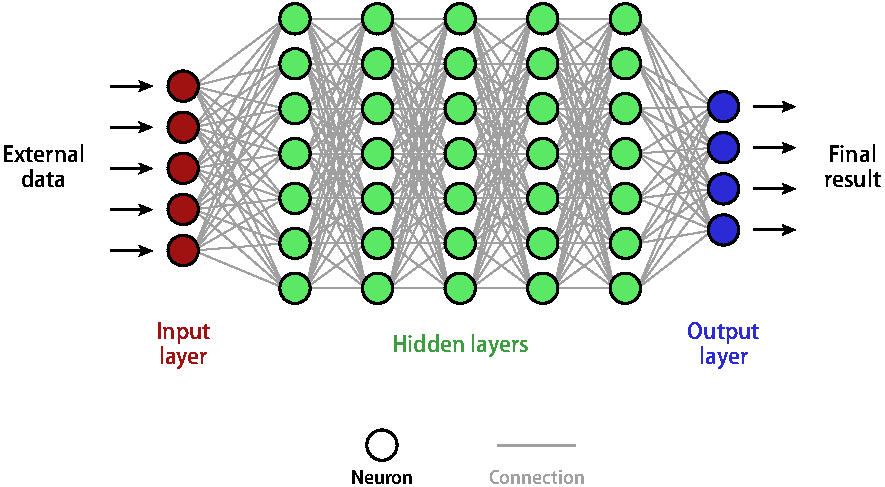
\includegraphics[width=125mm]{neural_network}
\caption{\label{fig:neural_network} Schematic representation of a deep neural network, a type of artificial neural network featuring several hidden layers of neurons between the input and output layers.}
\end{figure*}

In each of the hidden layers, the neurons receive the input signal from others neurons, process it by combining the input with their internal state, and produce an output signal. The neural network links these neurons through connections, providing the output of one neuron as an input to another neuron. Each neuron can have multiple input and output connections, to which are assigned weights, forming the overall layer of the NN. The learning process involves the adaptation of the network, \emph{i.e.} the weights of the connections, by minimizing the observed errors in the output of the neural network. Because of this very generic and self-adapting architecture of the NN, deep learning reduces need for feature engineering, and can identify and work around defects that would be difficult to spot in other techniques. However, the training of artificial neural networks requires a very large amount of data to train accurately, and is computationally expensive due to the large number (millions or more) of parameters to optimize during training.

Several research groups have proposed applications of deep learning to problems in chemical and materials sciences.\cite{Mater2019} For example, Willighagen et al. used supervised self-organizing maps (a kind of ANN) to explore large numbers of experimental and simulated crystal structures, in order to visualize structure-property relationships.\cite{Willighagen2007} Using ANN implemented in the open-source PyBrain code,\cite{pybrain2010jmlr} Ma et al. developed a model trained with a set of \emph{ab initio} adsorption energies and electronic fingerprints of idealized bimetallic surface among them spatial extent of metal $d$-orbitals, atomic radius, ionization potential, electron affinity and Pauling electronegativity.\cite{Ma2015} This model was able to captures complex non linear adsorbate--substrate interactions, as it is applied to the electrochemical reduction of carbon dioxide on metal electrodes.

Rules-based expert systems (rules are applied to the reactants to obtain the product in reaction prediction, or to the product for retrosynthesis) cannot predict outside of their knowledge and often fail because they ignore the molecular context, which leads to reactivity conflicts. To overcome this problem, deep learning techniques have been used to predict chemical synthesis routes by combining NN with rules-based expert systems. Using this combination, Segler et al. have ranked the candidate synthetic pathways by the compute of mean reciprocal rank (MRR).\cite{Segler2017} This model was trained on 3.5~million reactions with a success rate of {95\%} in retrosynthesis and {97\%} for reaction prediction. In another work, Cole et al. have determined the probability of the predicted product using more than 800,000  organic and organometallic crystal structures in the CSD Database.\cite{Cole2016} Deep learning is also used in the study and discovery of drug-like molecules, e.g., G{\'o}mez-Bombarelli et al. have estimated the chemical properties from the latent continuous vector representation of the molecule using RNN method.\cite{GomezBombarelli2018} The model they developed allows to generate new molecules for efficient exploration and optimization.


\section{Artificial intelligence in the lab}

While this paper is focused on providing an introductory description of machine learning approaches for the prediction of chemical systems in general, and materials properties more specifically, we want to end it by noting that the use of artificial intelligence techniques in chemistry and materials science is much broader than machine learning and its computational applications --- and it provides a lot of exciting avenues for research in the near future.\cite{AspuruGuzik2019} We refer the reader to Ref.~\citenum{deAlmeida2019} for an in-depth and very insightful review of the multiple avenues of research opened by artificial intelligence in the field of synthetic organic chemistry.

One particular area of recent achievements for artificial intelligence in chemistry is its integration into a chemistry labs achieved through robotics.\cite{Gromski2020} Robotic synthesis based on flow chemistry takes high-throughput discovery to an entirely new scale --- where chemical syntheses can be described through standardized methods descriptions, \emph{i.e.} ``source code for chemistry'', which is then compiled for the specific hardware of a synthesis robot.\cite{Steiner2019} Furthermore, this allows high-throughput synthesis and characterization to be tightly coupled with computational screening procedures.\cite{Greenaway2018} In this approach, it is thus possible to leverage an artificial intelligence algorithm to propose synthetic routes, coupled with a robotic microfluidic platform to realize the synthesis and characterize its results.\cite{Empel2019} To list two recent examples, Coley et al proposed a robotic platform for flow synthesis of organic compounds, paired with computational prediction techniques based on artificial intelligence.\cite{Coley2019} Granda et al. demonstrated an integrated system where machine learning is used for decision making in real time, during a trial-and-error search for new reactivity where analysis results from experiments are fed back into the ML algorithm.\cite{Granda2018}



\begin{acknowledgments}
A large part of the work discussed in this article requires access of scientists to large supercomputer centres. Although no original calculations were performed in the writing of this paper, we acknowledge GENCI for high-performance computing CPU time allocations (grant A0070807069). This work was funded by the Agence Nationale de la Recherche under project ``MATAREB'' (ANR-18-CE29-0009-01).
\end{acknowledgments}

\section*{Data Availability}
Data sharing is not applicable to this article as no new data were created or analyzed in this study.

\section*{References}
\bibliography{references}

\end{document}
